%\documentclass[a4paper, twocolumn]{article}
\documentclass[11pt]{article}
\pagestyle{empty}

\usepackage[a6paper]{geometry}
\usepackage[portuguese]{babel}
\usepackage[latin1]{inputenc}
\usepackage[T1]{fontenc}
\usepackage{pstricks}
\usepackage{pst-plot}
\usepackage[pdftex]{graphicx}
\usepackage{booktabs}
%\usepackage[top=1cm,bottom=1cm,left=1cm,right=1cm]{geometry}
%\usepackage{multicol}

\usepackage{amssymb,amsmath}
%\usepackage{extraipa}
\usepackage{euler}
\everymath{\displaystyle}

\DeclareMathOperator{\N}{\mathbb{N}}
\DeclareMathOperator{\Z}{\mathbb{Z}}
\DeclareMathOperator{\R}{\mathbb{R}}
\DeclareMathOperator{\negate}
    {\negthickspace\negthickspace\negthickspace\diagup\negthickspace}
\DeclareMathOperator{\dom}{dom}
\DeclareMathOperator{\im}{im}
\DeclareMathOperator{\proj}{proj}
\DeclareMathOperator{\sen}{sen}
\DeclareMathOperator{\tg}{tg}
\providecommand{\abs}[1]{\lvert#1\rvert}
\providecommand{\vt}[1]{\overrightarrow{#1}}
\newcommand{\xa}[1]{\renewcommand{\arraystretch}{#1}}

\author{Andr� Wagner}
\title{C�lculo}
\date{}

\begin{document}

\section{Vetores}

Se $\vec{v} = \vt{AB}$, ent�o $\vec{-v} = \vt{BA}$.
\[ \vec{u} + \vec{v} = (u_1+v_1, u_2+v_2) \]
\[ \vec{u} - \vec{v} = (u_1-v_1, u_2-v_2) \]
\[ a\vec{v} = (av_1, av_2) \]

Se $\theta$ � o �ngulo entre dois vetores $\vec{u}$ e $\vec{v}$ ent�o:
\begin{itemize}
  \item Se $\theta = 0$, ent�o $\vec{u} = \vec{-v}$;
  \item Se $\theta = \pi$, ent�o $\vec{u} = \vec{v}$;
  \item Se $\theta = \frac{\pi}{2}$, ent�o $\vec{u} \perp \vec{v}$;
  \item O �ngulo entre $\vec{u}$ e $-\vec{v}$ � $\pi-\theta$.
\end{itemize}

\[ \vt{AB} = B-A \]
\[ \vt{AB} = (x_2-x_1, y_2-y_1, \ldots) \]

Se $\vec{u} \parallel \vec{v}$, ent�o $\frac{x_1}{x_2} = \frac{y_1}{y_2} = \ldots$


\section{Produto de Vetores}

\[ \vec{u}\cdot\vec{v} = x_1 x_2 + y_1 y_2 + z_1 z_2 \]
\[ \vec{u}\cdot\vec{v} = \abs{\vec{u}}\abs{\vec{v}}\cos\theta \]
\[ \abs{\vec{u}}\abs{\vec{v}}\cos\theta = x_1 x_2 + y_1 y_2 + z_1 z_2 \]
\[ \cos\theta = \frac{\vec{u}\cdot\vec{v}}{\abs{\vec{u}}\abs{\vec{v}}} \]

\[ \abs{\vec{v}} = \sqrt{x^2+y^2+z^2} \]
\[ d = \sqrt{(x_2-x_1)^2 + (y_2-y_1)^2 + (z_2-z_1)^2} \]
\[ \proj_{\vec{v}} \vec{u} = \left( \vec{u} \cdot \frac{\vec{v}}{\abs{\vec{v}}} \right) \frac{\vec{v}}{\abs{\vec{v}}} \]
\[ \proj_{\vec{v}} \vec{u} = \left( \frac{\vec{u}\cdot\vec{v}}{\vec{v}\cdot\vec{v}} \right) \vec{v} \]

Se $ \vec{u}\cdot\vec{v} = 0 $, ent�o $ \vec{u}\perp\vec{v} $.

\section{Produto Vetorial}

\[ \vec{u}\times\vec{v} = \begin{vmatrix}
                            \vec{i} & \vec{j} & \vec{k} \\
                            x_1 & x_2 & x_3 \\
                            y_1 & y_2 & y_3
                          \end{vmatrix} \]
Se $ \vec{u}\times\vec{v} = \vec{0} $, ent�o $ \vec{u}\parallel\vec{v} $.


\begin{figure}
\centering
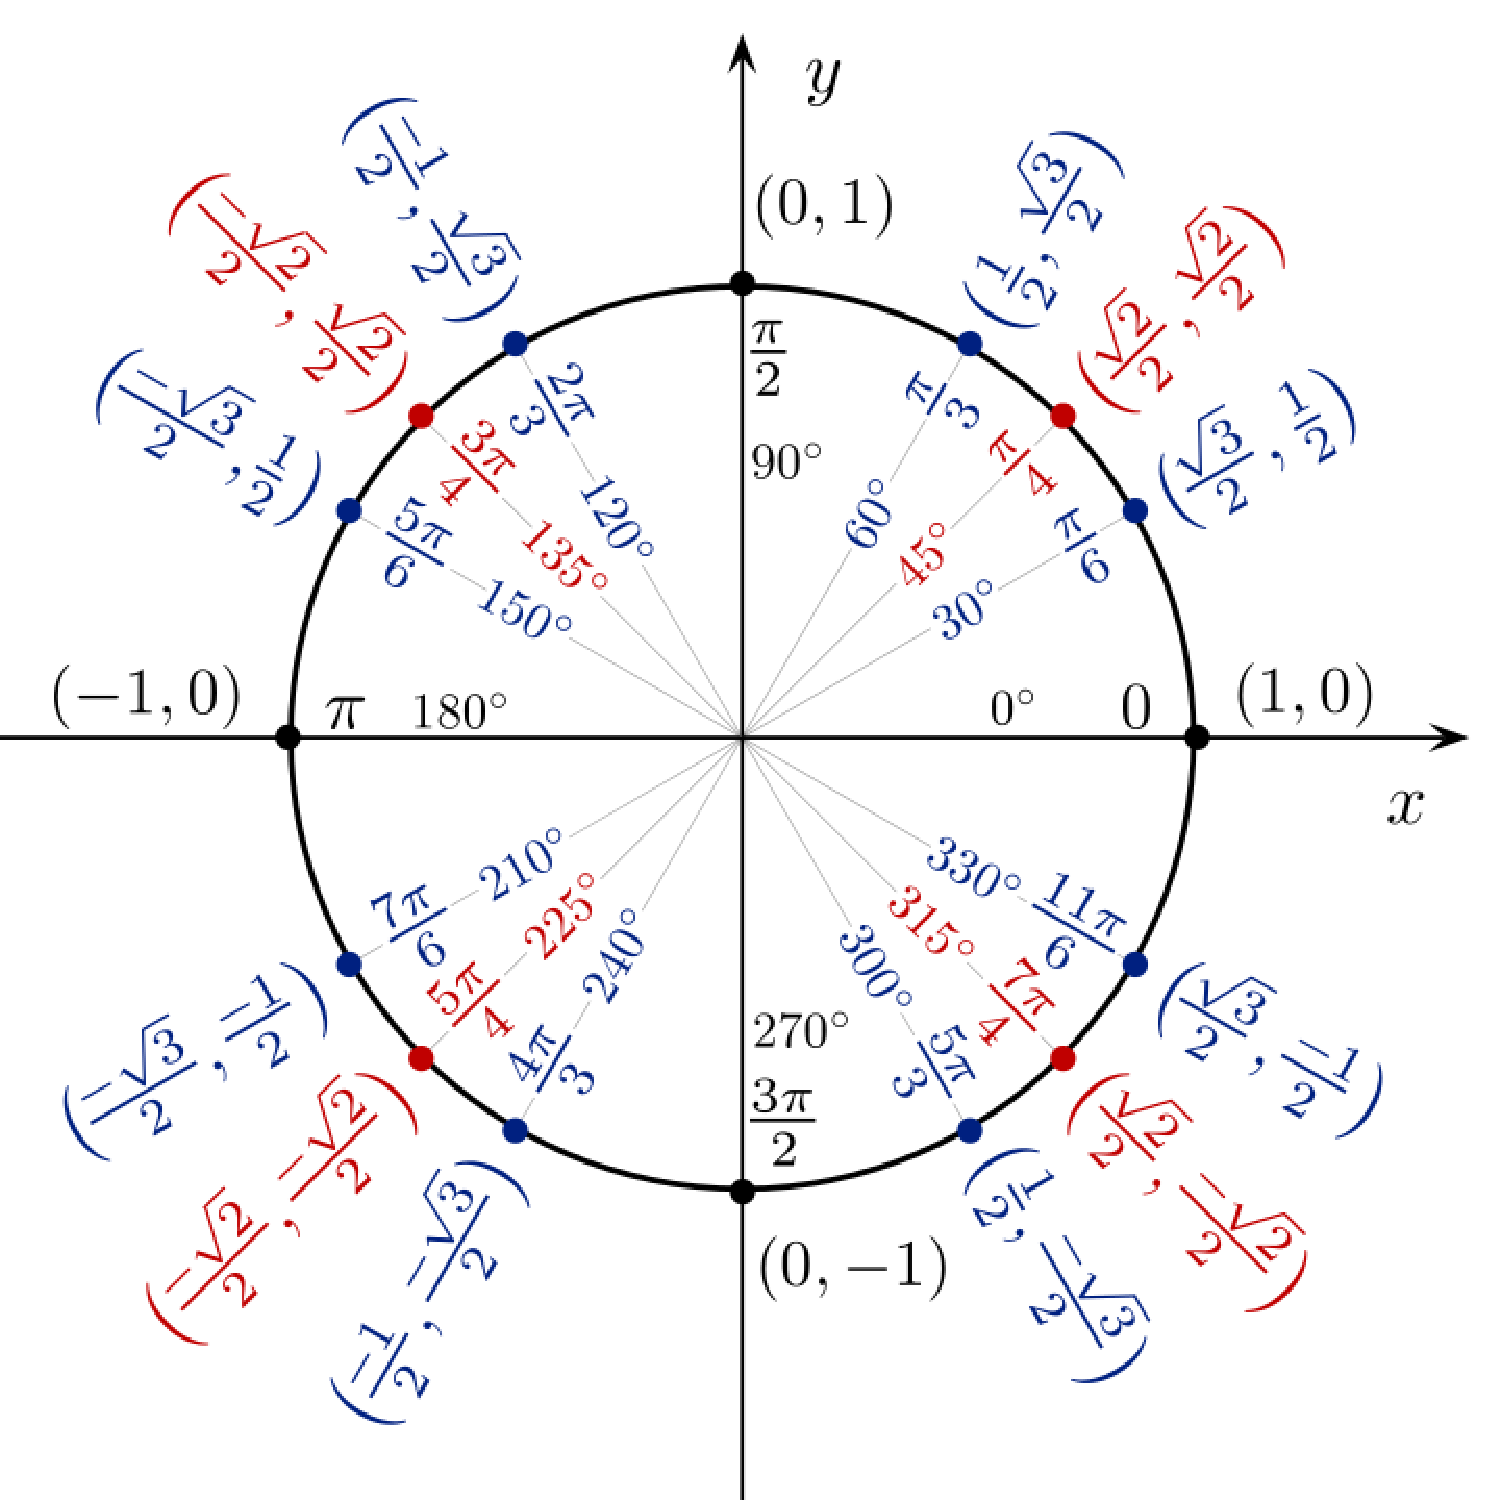
\includegraphics[scale=0.35]{Unit_circle_angles_color.pdf}
\end{figure}

\section{A Reta}

\[ \vec{x} = P + \lambda\vec{v} \]

onde $\vec{x}$ � a reta, $P$ � o ponto b�sico, $\lambda$ � o n�mero de passos
e $\vec{v}$ � o vetor diretor (que d� a dire��o da reta).

Reta que passa pelos pontos $A$ e $B$:

\[ \vec{x} = A + \lambda(B-A) \]

\[ PM = \frac{(u_1, u_2, u_3) + (v_1, v_2, v_3)}{2} \]

\section{Planos}

\[ \vec{x} = P + \lambda\vec{v} + \mu\vec{w} \]

\section{Circunfer�ncia}

\[ \sqrt{(x-c_1)^2 + (y-c_2)^2} = r \]

Onde $C(c_1,c_2)$ � o centro da circunfer�ncia, $P(x,y)$ os pontos por onde
passa a linha, e $r$ o raio.

\section{Elipse}

\[ \frac{(x-c_1)^2}{a^2} + \frac{(y-c_2)^2}{b^2} = 1 \]

Onde $a$ � a dist�ncia entre a lateral e o centro da elipse, e $b$ � a dist�ncia
entre o topo e o centro.

\section{Par�bola}

\[ y^2 = 4px: \subset \]
\[ y^2 = -4px: \supset \]
\[ x^2 = 4py: \cup \]
\[ x^2 = -4py: \cap \]

\section{Derivadas}

\[ f'(x) = \lim_{h \to 0} \frac{f(x+h) - f(x)}{h} \]

\[ (f \pm g)'(x) = f'(x) \pm g'(x) \]

\[ (\alpha f)'(x) = \alpha f'(x) \]

\[ (f \cdot g)'(x) = f'(x)g(x) + f(x)g'(x) \]

\[ \left(\frac{f}{g}\right)'(x) = \frac{f'(x)g(x)-f(x)g'(x)}{\left[g(x)\right]^2} \]

\[ \left[g(f(x))\right]' = g'\left(f(x)\right)f'(x) \]

\section{Reta tangente}

$\alpha$ � o ponto que se quer encontrar.

\[ y = f'(\alpha) \cdot (x - \alpha) + f(\alpha) \]

\section{Tabela de integrais e derivadas}

\begin{table*}\centering
\xa{1.3}
\begin{tabular}{@{}lll@{}}
\toprule
f'(x) & f(x) & $\int x$ \\ 
\midrule
$nx$ & $x^n$ & \\
$e^x$ & $e^x$ & \\
$\cos x$ & $\sen x$ & \\
$-\sen x$ & $\cos x$ & \\
$\sec^2 x$ & $\tg x$ & \\
$\sec x \tg x$ & $\sec x$ & \\
$n^x\log_e n$ & $n^x$ & \\
\bottomrule
\end{tabular}
\end{table*}

\end{document}
